Uživatelským požadavkem je dynamické zařízení sloužící například jako identifikátor hráče, nebo jako herní nástroj.
Mělo by ale být sto zastat i~roli statického zařízení, pro případy her na delších výletech, kde by bylo nepraktické nosit s~sebou velké zařízení.
Vyžaduje tedy dostatečnou mobilitu, aby uživateli nepřekáželo v~pohybu.
Zároveň by zařízení mělo být co nejlevnější, pro případ ztráty nebo poškození.
Z~toho plynou požadavky na velikost výslednou konstrukci zařízení.

Zařízení by mělo být schopno komunikovat s~ostatními zařízeními, ať už statickými nebo dynamickými.
Potřebuje také světelný výstup pro zobrazování herních stavů a~jednoduchý vstup pro ovládání.

Vstup bude realizován pomocí dvou tlačítek.

Světelný výstup bude realizován pomocí pěti inteligentních RGB LED.
Číslo pět bylo zvoleno jako maximální množství, které se pohodlně vleze vedle sebe na desku plošných spojů o~šířce mikrokontroleru ESP32-C3-MINI-1 \cite{ESP32C3}.
ESP32-C3-MINI-1 byl vybrán jakožto nejlevnější mikrokontroler z~rodiny ESP32, který má zároveň Wi-Fi a~Bluetooth.

Abychom se vyhnuli elektronice řešící baterii, je napájení zajištěno pomocí USB-A konektoru a~powerbanky.

ESP32-C3-MINI-1 má stejně jako ESP32-S3 USB periferii, která se dá využít na programování zařízení.
I~tady je ale problém, že se tato metoda dá softwarově rozbít a~zařízení je proto vybaveno stejným programovacím konektorem jako ESP32-S3 na AHS.

% \section{Neočekávané problémy}
% První verce trpěla nečekaným problémem s~kmitajícími hranami řídícího signálu LEDek.
% Tento problém pravděpodobně nastal v~důsledku kombinace parazitních vlastnosti výstupního pinu mikrokontroleru, vstupního pinu LEDek a~příliš krátké dráhy.

% Signál tak začal oscilovat na frekvenci zhruba \(50\-[MHz]\) a~LEDky tak nebyly schopny signál rozpoznat.
% \begin{tikzpicture}
%     \begin{axis}[
%         xlabel={X},
%         ylabel={Y},
%     ]
%     \addplot table [
%         x=x, 
%         y=y,
%         mark = none, 
%         col sep=comma
%     ] 
%     {text/PraktickaCast/img/zignalNaSemiSemaforu.csv};
%     \end{axis}
% \end{tikzpicture}


%%TODO: Ferit

% \begin{figure}[h]
%     \begin{minipage}[r]{0.5\textwidth}
%         \centering
%         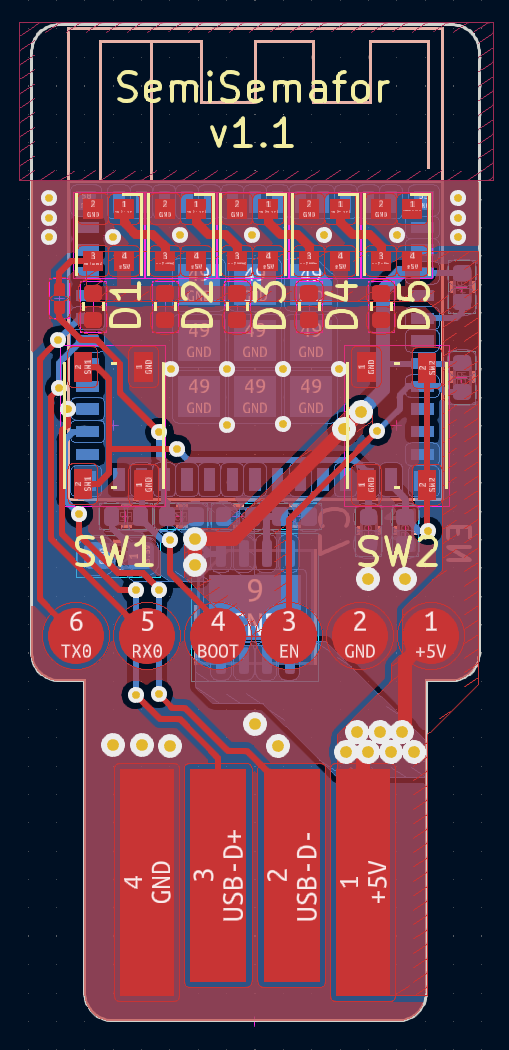
\includegraphics[width=\textwidth]{text/PraktickaCast/img/SemiSemafor-PCB.png}
%         \caption{Vzhled desky plošných spojů}
%         \label{fig:3D}
%     \end{minipage}
% \end{figure}
